\documentclass[12pt]{article}

\usepackage{enumerate}
\usepackage{rotating}
\usepackage{multicol}
\usepackage{multirow}
\usepackage{graphicx}
\usepackage{fullpage}
\usepackage{subfigure}
\usepackage{setspace}
\usepackage{listings}
\usepackage{lastpage}

\graphicspath{{./images/}}

% for references
\usepackage[pagebackref=false,colorlinks,linkcolor=blue,citecolor=magenta]{hyperref}
\usepackage[nottoc]{tocbibind}
\usepackage{fancyhdr}
\setlength{\headsep}{25pt}

\pagestyle{fancy}
\fancyhf{}
\lhead{\lr{Digital Image Processing}}
\rhead{تمرین سوم}
\cfoot{صفحه \thepage\ از \pageref{LastPage}}
\lfoot{نیمسال مهر 00-99}
\rfoot{حمیدرضا ابوئی مهریزی}


% xepersian
\usepackage[extrafootnotefeatures]{xepersian}
\settextfont[Scale=1.4]{B Nazanin}
\setlatintextfont{Times New Roman}

\renewcommand{\labelitemi}{$\bullet$}

\begin{document}
	\doublespacing
	\begin{titlepage}
		\paragraph*{}
		\centering
			
			
			{\small به نام او}\\
			\vspace{1cm}
			\includegraphics[width=0.12\paperwidth]{aut.png}
			\hspace{1cm}
			\includegraphics[width=0.15\paperwidth]{DIP}
			\hspace{1cm}
			\includegraphics[width=0.12\paperwidth]{bme}\\
			\vspace{2cm}
			{\Huge پردازش تصویر}\\
			\vspace{2cm}
			{\large استاد : دکتر حامد آذرنوش}\\
			\vspace{0.5cm}
			{\small  دانشجو :‌ حمیدرضا ابوئی}\\
			\vspace{0.5cm}
			{\small شماره دانشجویی : 9733002}\\
			\vspace{0.5cm}
			{\small تمرین سوم}\\
			\vfill
			{\tiny نیمسال مهر 00-99}
	\end{titlepage}
	\thispagestyle{plain}
	\tableofcontents
	\newpage
	%\onehalfspacing
	\doublespacing
	\section{سوال اول}
		\subsection{توضیحات تکمیلی روند کد}
		\lr{fftshift}
		یک دستور است که عملیات 
		\lr{centering}
		را برای ما انجام می‌دهد برای مثال همانگونه که در تصویر خروجی میبینید نقطه ی مرکز تصویر در وسط قرار گرفته است . این نقطه ، نقطه ی مهمی است که تمام فوکوس تصویر روی آن است و برای بهتر دیده شدن ما سعی داریم آن را در مرکز نمایش دهیم.
		 
		 همجنین لازم به ذکر است که تصویر 
		 \lr{Magnitude spectrum}
		 در اصل از طیف گسترده ای تشکیل شده است و ما با استفاده از لگاریتم گیری میتوانیم به این وضوح از تصویر برسیم.
		 فاز نیز بین 
		 $\frac{-\pi}{2}$
		 و 
		 $\frac{\pi}{2}$
		 تغییر میکند.
		 همچنین آینه کردن حول مرکز آینه به معنای چرخاندن ۱۸۰ درجه ای می باشد که با استفاده از قرینه کردن فاز تصویر امکان پذیر است .
		
	
		\subsection{ورودی برنامه}
		\includegraphics[width=5cm]{images/inputs/chest.png}
		\subsection{خروجی برنامه}
		
		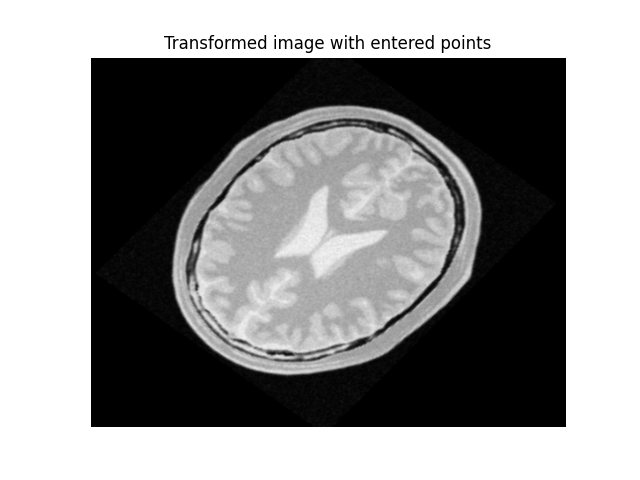
\includegraphics[width=15cm]{images/1.png}
		\newpage
		
		\section{سوال دوم}
		\subsection{توضیحات تکمیلی روند کد}
		برای تابع ، ورودی های خواسته شده و همچنین برای فیلتر باترورث نیاز به یک ورودی 
		\lr{D0}
		نیز داریم که می توانیم به صورت یک ورودی اختیاری وارد کنیم . و مقدار اولیه ی آن را همانطور که دیدیم و بهینه ی آن عدد ۲ است ، دو وارد میکنیم.
		در این کد سعی شده است که برای هر فیلتری  که با استفاده از یک شرط مشخص می‌شود. فیلتر مورد نیاز برای آن فیلتر را جداگانه حساب کند و سپس آن را به تصویر زیروپدینگ شده اعمال نماییم. و سپس تصویر فیلتر شده را بازسازی می‌کنیم .
	حال همانطور که در تصاویر خروجی مشخص است و از تبدیل فوریه انتظار داشتیم، میزان رینگینگ در فیلتر ایده آل زیاد است زیرا به سینک تبدیل می‌شود اما در فیلتر باترورث این رینگینگ کاهش می‌یابد و در فیلتر گاوسین این رینگینگ حذف می‌شود زیرا ماهیت فیلتر گاوسین 
	\lr{exp}
	می باشد که در اثر انتگرال و مشتق تغییر ماهیت نمی‌دهد.
	
		\subsection{ورودی برنامه}
		\includegraphics[width=5cm]{images/inputs/a.png}
		\subsection{خروجی برنامه}
		
		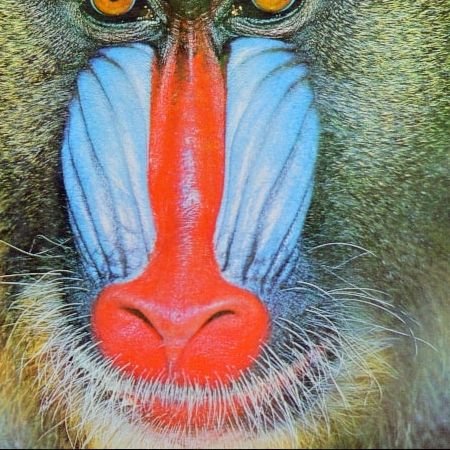
\includegraphics[width=18cm]{images/2.png}
		\newpage
		
		\section{سوال سوم}
		\subsection{توضیحات تکمیلی روند کد}
			همانگونه که در تصویر مشخص است، به نظر می‌رسد که در خروجی، فاز تعیین کننده ی اصلی جزئیات تصویر می‌باشد ولی به صورت کامل تصویر تشکیل نمی‌شود و دامنه در نقش ایجاد کننده و مشخص کننده ی  طیف های تصویر است. 
			در اصل مهم تر فاز است که اصل تصویر را تشکیل میدهد و لازم است که حفظ شود و با تغییرات در دامنه ، به تصویر مورد نظر برسیم.
	
	
		\subsection{ورودی برنامه}
		
		\includegraphics[width=5cm]{images/inputs/clown.png}
		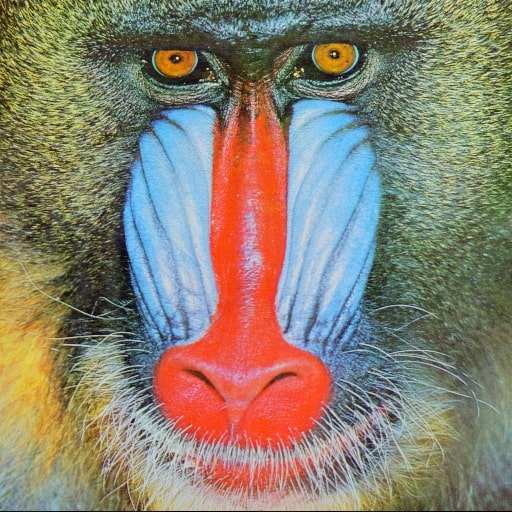
\includegraphics[width=5cm]{images/inputs/mandrill.png}
		
		\subsection{خروجی برنامه}
		
		\includegraphics[width=16cm]{images/3.png}
		\newpage
		

\end{document}
